\documentclass[a4paper, 11pt, onecolumn, oneside]{report}

\setcounter{tocdepth}{3} % Para aparecer no índice subsubsections
\setcounter{secnumdepth}{3} % Para subsubsections serem numeradas

%%%%% Funcionalidades %%%%%
\usepackage[T1]{fontenc} % Fontes T1
\usepackage[utf8]{inputenc} % Input UTF8
\usepackage[backend=biber, style=ieee]{biblatex} % para usar bibliografia
\usepackage{csquotes}
\usepackage[portuguese]{babel} % Usar língua portuguesa
\usepackage{blindtext} % Gerar texto automaticamente
\usepackage[printonlyused]{acronym} % Para lista de acrónimos
\usepackage{hyperref} % para autoref
\usepackage{graphicx} % Suporte para gráficos2
\usepackage{indentfirst}  % Indentação automática em secções
\usepackage{wrapfig} % Imagens junto do texto
\usepackage{enumitem} % Para usar em enumerações
\usepackage{tabularray} % Alinhar conteudos tabelas
    \UseTblrLibrary{booktabs, varwidth}


\bibliography{bibliografia}
\graphicspath{{images/}} % Diretório com as Imagens



%%%%%%%%%%%%%%%%%%%%%%%%%%%%%%%%%%%%%%%%%%%%%%%%%%%%%%%%
\begin{document}
%%
% Definições
%
\def\titulo{Impacto da Inteligência Artificial}
\def\data{DATA}
\def\autores{Tiago Mendes, Paulo Lacerda}
\def\autorescontactos{(119378) tfdmendes@ua.pt, (120202) paulolacerda@ua.pt}
\def\versao{1}\def\repositorio{infor2023-ap-g-infor2023-ap-g16}
\def\departamento{Dpt. de Eletrónica, Telecomunicações e Informática}
\def\empresa{Universidade de Aveiro}
\def\logotipo{ua.pdf}
%
%%%%%% CAPA %%%%%%
%
\begin{titlepage}

\begin{center}
%
\vspace*{50mm}
%
{\Huge \titulo}\\ 
%
\vspace{10mm}
%
{\Large \empresa}\\
%
\vspace{10mm}
%
{\LARGE \autores}\\ 
%
\vspace{30mm}
%
\begin{figure}[h]
\center
\includegraphics{\logotipo}
\end{figure}
%
\vspace{30mm}
\end{center}
%
\begin{flushright}
\versao
\end{flushright}
\end{titlepage}

%%  Página de Título %%
\title{%
{\Huge\textbf{\titulo}}\\
{\Large \departamento\\ \empresa}
}
%
\author{%
    \autores \\
    \autorescontactos
}
%
\date{\today}
%
\maketitle

\pagenumbering{roman} % Numeração Romana para as páginas seguintes

%%%%%% RESUMO %%%%%%
\begin{abstract}
\textbf{Este trabalho aborda o campo de Inteligência Artificial, em particular a sua evolução, impacto parcial ao longo da história, e a respetiva responsabilidade ética aquando do seu uso.}
\par
Através de métodos de pesquisa baseados em análise de artigos científicos e fontes profissionais, foi possivel criar o documento em causa, com o objetivo de esclarecer o desenvolvimento de inteligência artificial ao longo do tempo e a sua relação com as transformações na criação de sistemas inteligentes, e as suas aplicabilidades éticas.
Desta maneira, são destacados os desafios e oportunidades futuras, incluindo a perspetiva de inteligência artificial, regulamentação governamental, aspéticos éticos em conta e o impacto potencial no mercado de trabalho. Oferece uma visão extensa da evolução da inteligência artificial, desde as suas origens até às tendências atuais e futuras. 
\par
Em última análise, a evolução da inteligência artificial é uma narrativa de progresso e desafios contínuos, prometendo  transformações incessantes na sociedade. Este documento será então um guia para entender essa jornada e para antecipar caminhos que inteligência artificial possa vossa vir a trilhar no futuro.
\end{abstract}

%%%%%% Agradecimentos %%%%%%
% Segundo glisc deveria aparecer após conclusão...
% \renewcommand{\abstractname}{Agradecimentos}
% \begin{abstract}
% Comentou-se este bloco devido à falta de agradecimentos a fazer.
% \end{abstract}

\renewcommand{\contentsname}{Índice}
\tableofcontents
%%%%%%%%%%%%%%%%%%%%%%%%%%%%%%%%%%%%%%%%%%%%%%%%%%%%%%%%
%%%%%% Indice de Tabelas %%%%%%
\listoftables

%%%%%%%%%%%%%%%%%%%%%%%%%%%%%%%%%%%%%%%%%%%%%%%%%%%%%%%%
%%%%%% Indice de Imagens %%%%%%
\listoffigures

%%%%%%%%%%%%%%%%%%%%%%%%%%%%%%%%%%%%%%%%%%%%%%%%%%%%
\clearpage
\pagenumbering{arabic}
%
%%%%%%%%%%%%%%%% Introdução %%%%%%%%%%%%%%%%
\chapter{Introdução}
\label{chap.introducao}

%%%%% O que é? %%%%%
\section{O que é inteligência artificial?}
\ac{ia}\cite{artificial_intelligence} é a capacidade de computadores ou programas de software de realizarem tarefas que normalmente requerem a intervenção humana. Estes sistemas são projetados para simular a inteligência humana, incluindo o raciocínio, aprendizagem, resolução de problemas e capacidade de decisão. Inteligência artificial utiliza algoritmos e modelos matemáticos para processar dados e realizar ações com base no processamento dessas características humanas.

%%%%% Importância %%%%%
\section{Importância}
Esta tecnologia revoluciona a maneira como é possível abordar desafios específicos em diversos setores, desde a saúde até ao setor financeiro, promovendo eficiência e inovação. \ac{ia} automatiza tarefas rotineiras, permitindo que profissionais se concentrem em atividades mais criativas e complexas. Em simultâneo, a capacidade da \ac{ia} de analisar grandes volumes de dados e identificar padrões contribui para a toma de decisões mais fundamentadas. 
\par
Em áreas como a saúde, aprimora diagnósticos médicos e auxilia na pesquisa de novos tratamentos. No setor de mobilidade, contribui para o desenvolvimento de veículos autónomos e otimiza a gestão do tráfego. Oferece oportunidades económicas, criando empregos e estimulando a inovação. 
\par 
No entanto, apesar de todas as vantagens, é essencial abordar questões éticas e de segurança à medida que implementamos esta tecnologia, garantindo que a sociedade beneficia de maneira responsável e equitativa.

%%%%% Objetivo %%%%%
\section{Objetivo}
O objetivo deste trabalho é destacar a importância e o impacto da \ac{ia} e como a implementação dessa tecnologia pode afetar positivamente ou negativamente as operações de inteiros setores. Procura igualmente, estabelecer uma linha de tempo precisa sobre os acontecimentos no mesmo. Além disso procura enfatizar a relevância e responsabilidade ética na sua adoção, garantindo que as soluções baseadas na mesma sejam desenvolvidas e utilizadas de forma justa e equitativa, tendo em consideração questões como a privacidade e transparência.
\par 
A \ac{ia} é uma ferramenta poderosa que pode impulsionar a eficiência e a inovação, mas é fundamental compreender as implicações éticas e impactos sociais associadas ao seu uso. Portanto, um dos objetivos deste trabalho é também promover uma compreensão mais profunda da \ac{ia} e as suas implicações, incentivando uma adoção responsável e benéfica para a sociedade e negócios.

%%%%% Metodologia %%%%%
\section{Metodologia}
A abordagem à realização deste documento seguiu um conjunto de etapas.
\par 
Uma revisão extensa e constante da literatura relevante. Isso envolveu a análise de livros, relatórios e artigos científicos. Essa revisão providenciou bases técnicas para entender os conceitos-chave e tendências relacionadas com impacto \ac{ia}.
%%%%% Estrutura %%%%%
\section{Estrutura do Documento}
Este documento está subdividido em 5 capítulos, com um total de 22 secções, 5 subsecções e ainda 6 sub-subsecções. 
\par
Breve explicação sobre a informação de cada capítulo:
\begin{enumerate}
    \item Pequena introdução sobre o documento;
    \item Oferece uma Cronologia sobre marcos importantes na Inteligência artificial;
    \item Os diferentes impactos que Inteligência Artificial poderá ter(tem) em alguns setores;
    \item Aspetos éticos relacionados com a utilização da inteligência artificial;
    \item Conclusão do documento.
\end{enumerate}
%
%%%%%%%%%%%%%%%%%%% Percurso IA %%%%%%%%%%%%%%%%%%%%%%%%%%%
%
\chapter{Percurso da Inteligência Artificial}
\label{chap.origens}
O percurso da inteligência artificial (IA) é uma jornada fascinante que se estende ao longo de décadas, com avanços significativos em diversas áreas. 

%%%%% Primórdios %%%%%
\section{Primórdios: 1900-1950}
No inicio dos anos 1900, diferentes meios de mídia divulgaram a ideia que seres humanos artificiais. Tanto é que diferentes cientistas de várias áreas começaram a fazer a pergunta se de facto seria possível criar um cérebro artificial. Ideia que posteriormente evoluiu para o termo atual, "robôs".
%
\begin{itemize}
    \item \textbf{1921:} Karel Čapek publica a peça de teatro "Rossum's Universal Robots"\cite{rossum_universal_robots}. Introduz a ideia de seres humanos artificiais, que ele intitulou de "robôs". Esta foi a primeira aparição da palavra.
    %
    \item \textbf{1929:} Professor japonês Makoto Nishimura constrói o primeiro robô japonês, \textit{Gakutensoku}\cite{gakutensokus}
\end{itemize}

%%%%% Nascimento %%%%%
\section{Nascimento: 1950-1956}
Este período de tempo foi quando surgiu o interesse por Inteligência Artificial.
%
\begin{itemize}
    \item \textbf{1950:} Alan Turning, um dos pioneiros da ciência de computação britânica, publicou “Computer Machinery and Intelligence”\cite{alan_turning}
    %
    \item \textbf{1952:} Arthur Samuel, cientista de computação britânico, desenvolve um programa para jogar damas, sendo o primeiro a aprender o jogo de forma independente, e primeiro vestígio de inteligência artificial.
\end{itemize}
\par
O termo de inteligência artificial foi cunhado na Conferência de Dartmouth, em 1956, nos Estados Unidos. Esta conferência marcou, formalmente, a inteligência artificial como um campo de estudo 

%%%%% Amadurecimento %%%%%
\section{Amadurecimento: 1957-1979}
O período entre a criação da expressão "inteligência artificial" e a década de 1980 foi um período de desafios e rápido crescimento para a pesquisa em IA. O final dos anos 1950 até à década de 1960 foi uma época de criação. Desde linguagens de programação que ainda são usadas até hoje, até livros e filmes que exploraram a ideia de robôs, a IA rapidamente se tornou uma ideia convencional.

%
\begin{itemize}
    \item \textbf{1959:} Arthur Samuel cria o termo Machine Learning\footnote{Uso de dados específicos para fazer previsões e recomendações sobre como alcançar objetivos declarados.} ao proferir uma palestra sobre ensinar máquinas a jogar xadrez melhor do que os humanos que as programaram.
    %
    \item \textbf{1961:} O primeiro robô industrial, chamado \textit{Unimate}, começa a trabalhar numa linha de montagem na General Motors, em Nova Jersey, encarregado de transportar carcaças de matrizes e soldar peças em carros (uma tarefa considerada demasiado perigosa para humanos)
    %
    \item \textbf{1979:} James L. Andams cria, em 1961, o primeiro exemplo de veículo autónomo, \textit{The Stanford Cart}\cite{stanford_cart}. Em \textit{'79}, navegou com sucesso por uma sala cheia de cadeiras sem intervenção humana.
\end{itemize}

%
\begin{figure}[ht]
    \centering
    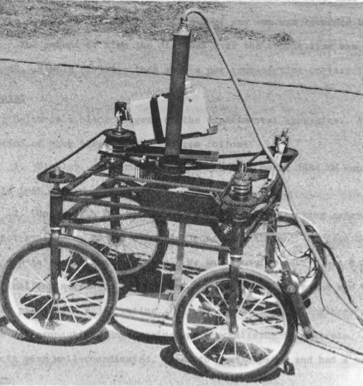
\includegraphics[scale=0.35]{images/stanford_car.png}
    \caption{Stanford Car\cite{i21}}
    \label{stanford_car}
\end{figure}
%

\newpage %forçar nova página

%%%%% Inverno IA %%%%%
\section{Inverno da IA: 1987-1993}
A maior parte deste período é referida como o "Inverno da \ac{ia}", indicando uma época de financiamento e interesse reduzidos e, consequentemente, menos desenvolvimentos significativos. Muitos reconhecem dois invernos principais: o primeiro no final da década de 1970, impulsionado pelas percebidas limitações da tecnologia, e o segundo no final da década de 1980 até o início da década de 1990, motivado pelos custos excessivos no desenvolvimento e manutenção de bancos de dados digitais especializados. Apesar da falta de interesse geral durante este período, a colaboração entre os pioneiros no campo, continuou.

%%%%% Presente %%%%%
\section{Presente: 2012-2023}
Inteligência Artificial representa um multiplicador/impulsionador de força no progresso tecnológico, servindo de alicerce para fomentar outras tecnologias, estimular desenvolvimento de negócios, governos e sociedades.
%
\begin{itemize}
    \item \textbf{2012:} O \textit{Google Brain}\cite{google_brain}, uma equipa de pesquisa liderada pelos pesquisadores da Google Jeff Dean e Andrew Ng, através de métodos como Machine Learning "treinam" uma rede neural para reconhecer gatos baseado em 10 milhões de imagens digitais tiradas de vídeos do Youtube. 
    %
    \item \textbf{2015:} A \textit{AlphaGo}\cite{alphago}, uma inteligência artificial desenvolvida pela DeepMind, vence o campeão mundial de Go\footnote{Jogo de estratégia}, Lee Sedol, representando um avanço notável em jogos estratégicos.
    %
    \item \textbf{2019:} A OpenAI lança o modelo de linguagem \ac{gpt2}, evidenciando uma capacidade notável de gerar texto coerente e convincente.
    %
    \item \textbf{2020:} A OpenAI lança o modelo de linguagem \ac{gpt3}    
\end{itemize}

%%% IA em 2023 %%%
\subsection{IA em 2023}
ChatGPT\cite{chatpgt}, o chatbot viral da OpenAI que utiliza inteligência artificial para gerar conteúdo, despertou tanto interesse como preocupação no final de 2022, consolidando-se como o sistema de AI mais poderoso disponibilizado ao público. De uso facilitado, combinado com sugestões cada vez mais criativas, tornou-se dos maiores fenómenos globais. Criado pela mesma empresa responsável pelo desenvolvimento de \ac{gpt3} e do gerador de imagens \mbox{DALL-E 2}, o bot incitou reuniões de conselhos escolares que questionavam o uso do mesmo na entrega de trabalhos de casa \textit{supercharged}\footnote{sobrecarregado}, assustou investidores que questionavam o possível fim de métodos de pesquisa tradicionais, como o Google.
%
\begin{figure}[ht]
    \centering
    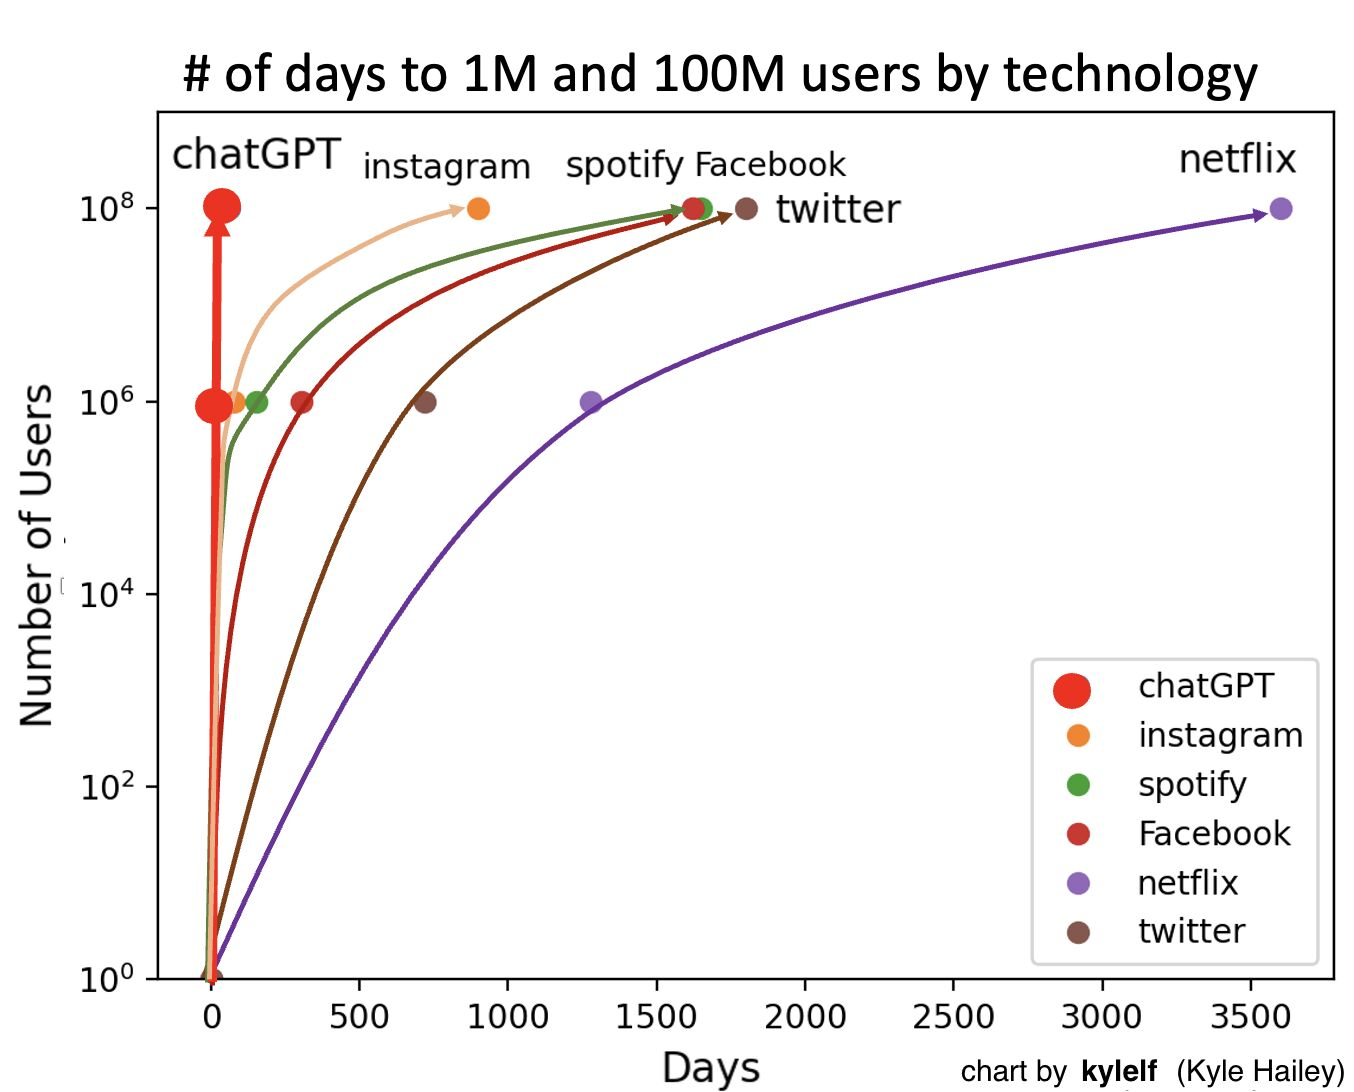
\includegraphics[scale=0.45]{images/chatgpt.jpg}
    \caption{Numero de dias até os 100 milhões de utilizadores\cite{i22}}
    \label{chatgpt_user_count}
\end{figure}
%
\par
\ac{ia} é atualmente usada em praticamente todas as indústrias, resolvendo desafios empresariais, detetando fraudes, otimizando rendimentos agrícolas, oferecendo recomendações e suporte a designers e escritores em tarefas criativas.  
\par
Por fim, a \ac{ia} não apenas resolve problemas existentes, mas também abre portas para oportunidades inovadoras, impulsionando o progresso em direções anteriormente inexploradas.


%%%%%%%%%% Futuro %%%%%%%%%%
\section{Futuro}
Conforme avançamos em rumo ao futuro, a \ac{ia} está fadada integrar-se ainda mais na sociedade. É natural antecipar uma \ac{ia} cada vez mais adaptativa, independente, e capaz de se ajustar dinamicamente às transformações do ambiente que a rodeia. A sua presença, eventualmente, será ubíqua, incorporada de raiz em diversos dispositivos e sistemas, promovendo uma experiência mais interconectada e fluída.

%%%%% Previsões %%%%%
\subsection{Previsões}
Prever o futuro da inteligência artificial é desafiador, mas com base nas tendências atuais e nas áreas de pesquisa em andamento é possível fazer algumas especulações razoáveis, tais como:

%%% QML %%%
\subsubsection{Computação Quântica e Machine Learning}
%
\begin{wrapfigure}{r}{0.33\textwidth}
    
\includegraphics[width=\linewidth]{images/qml.jpg}
    \caption{Quantum Machine Learning\cite{i23}}
    \vspace{4mm}
    \label{qml}
\end{wrapfigure}
%
A computação quântica é uma área emergente da computação que utiliza os princípios da mecânica quântica para processar informações. Enquanto que os computadores clássicos utilizam bits para representar informações, os computadores quânticos usam \textbf{qubits}\footnote{unidade básica de informação em computação quântica}, que podem existir em estados de 0, 1 ou ambos simultaneamente, graças ao fenómeno da superposição quântica.
\par
A interseção entre computação quântica e machine learning, conhecida como \ac{qml}, oferece várias possibilidades e potenciais impactos. Desde altas velocidade de processamento, desenvolvimento autónomo de algoritmos quânticos específicos, até à aprendizagem não supervisionada. Em \ac{qml}, são projetados circuitos quânticos para realizar tarefas específicas de aprendizado de máquina. Esses circuitos exploram a capacidade de qubits existirem em estados de superposição e entrelaçamento para realizar cálculos de forma paralela, potencialmente acelerando certos tipos de tarefas. 
\par
No entanto, apesar das diversas possibilidades que surgirão da integração entre machine learning e computação quântica, existem desafios que terão de ser superados até lá. Os computadores quânticos ainda apresentam falta de hardware quântico robusto, isto resulta num limite no número de qubits, que impede, por exemplo, a implementação de redes neurais complexas, ou algoritmos de \ac{ia} em grande escala.

%%% Desenvolvimento Ético %%%
\subsubsection{Desenvolvimento Ético e Regulamentação Rigorosa}
À medida que \ac{ia} se difunde mais na sociedade, as questões éticas relacionadas com o seu uso irão se destacar. A expectativa é que haja um aumento na implementação de regulamentações e padrões éticos para orientar o desenvolvimento e o uso responsável da mesma.

%%% XAI %%%
\subsubsection{Inteligência Artificial Explicável}
\ac{xai} ou, em português, Inteligência Artificial Explicável, é um conjunto de processos e métodos que permitem o ser humano compreender e confiar nos resultados criados por algoritmos de machine learning. A demanda de \ac{xai} irá aumentar à medida que a transparência e a compreensão das decisões tomadas por AI se tornarem essenciais. A capacidade de explicar o raciocínio por trás das decisões tomadas por IA será uma área de foco.
%
\begin{figure}[ht]
    \centering
    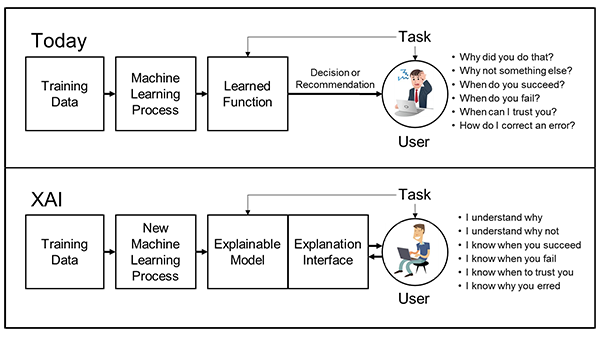
\includegraphics[scale=1.2]{images/xai.png}
    \caption{Representação Visual de XAI \cite{i24}}
    \label{xai}
\end{figure}

%
%%%%%%%%%%%%%%%%%% Impacto nos Setores %%%%%%%%%%%%%%%%%%
%
\chapter{Impacto nos Setores}
\label{chap.impacto_setores}

%%%%% Procura por  Talento %%%%%
\section{A rápida procura por talento}
Atualmente, mais que nunca, a procura por talento em IA ultrapassou a oferta. Nos Estados Unidos, houve quase três vezes mais anúncios de emprego relacionados com \ac{ia}\cite{ai_jobs} no ano passado do que de empregos para funções não relacionadas com \ac{ia}. Embora as escolas estejam a adicionar programas, a aumentar a inscrição e a incluir mais disciplinas para fundamentar os alunos dos conceitos básicos, a procura por competências em IA é simplesmente demasiado elevada e ainda existe uma escassez significativa de trabalhadores qualificados. O processo de contratação para ofertas de emprego em IA está a tornar-se mais demorado e dispendioso, prejudicando o futuro financeiro de algumas empresas.
%
\begin{figure}[ht]
    \centering
    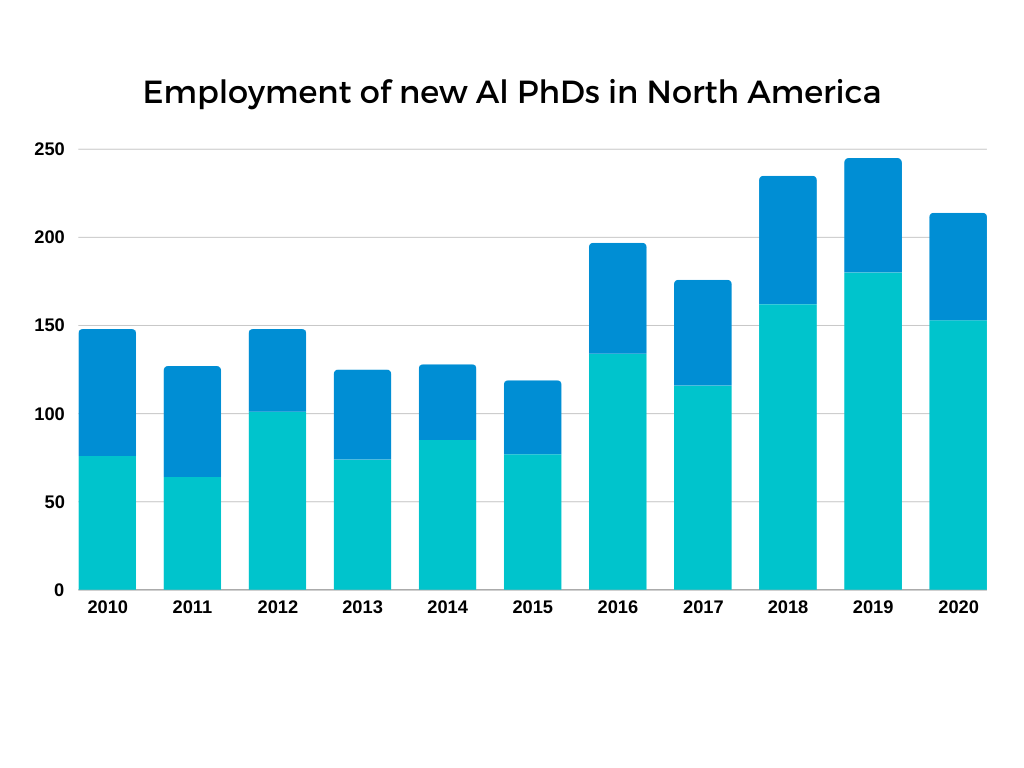
\includegraphics[scale=0.35]{images/employment.png}
    \caption{Taxa de Empregabilidade de Doutoramentos em IA\cite{i31}}
    \label{employment}
\end{figure}
%
\par
Inúmeras empresas estão a procurar melhorar as suas competências de trabalho em machine learning e em princípios básicos de IA. Como resultado, têm surgido numerosos programas de formação para ampliar o conhecimento, as competências, e as habilidades necessárias numa organização moderna. Levi Strauss lançou um \textit{bootcamp}\footnote{Campo de treino} de aprendizagem automática para aprimorar as competências da sua força de trabalho, ensinando aos funcionários como aplicar o pensamento de IA às tarefas do quotidiano. Fundada por professores da Universidade Harvard e da Universidade da Califórnia, Los Angeles, a \href{https://univ.ai/}{Univ.AI} é um programa online de formação em aprendizagem automática e IA.

%%%%% Saúde %%%%%
\section{Saúde}
%
\begin{wrapfigure}{l}{0.5\textwidth}
    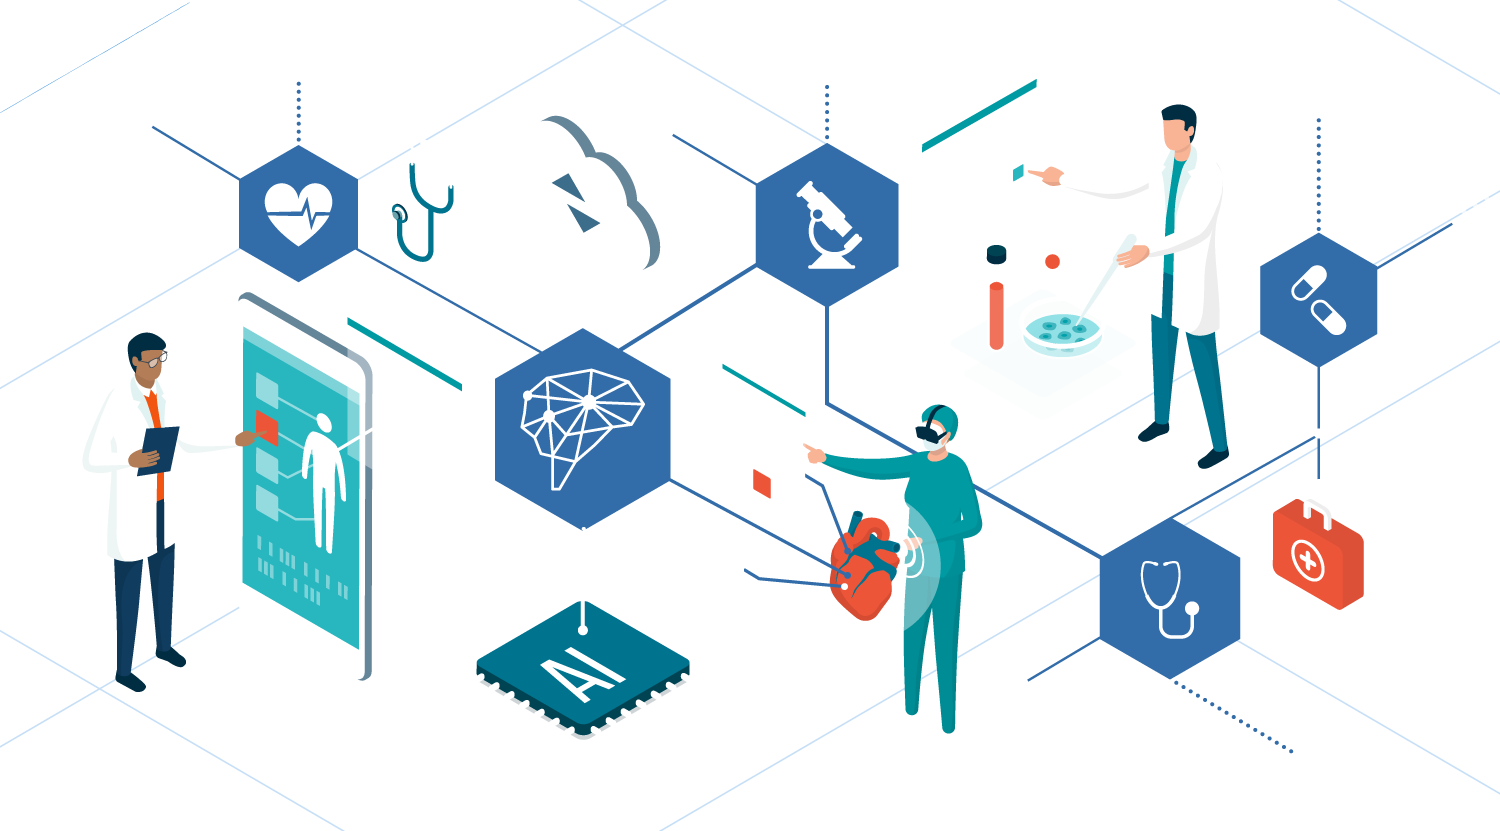
\includegraphics[width=\linewidth]{images/ai_health.png}
    \caption{Ilustração da \ac{ia} na saúde\cite{i32}}
    \vspace{4mm}
    \label{ai_health}
\end{wrapfigure}
%
A integração de Inteligência Artificial é fundamental no futuro da indústria da saúde. O foco primordial de toda a indústria da saúde tem sido a recolha de dados precisos e pertinentes sobre os pacientes, e aqueles que procuram tratamento. Consequentemente, a \ac{ia}  é um candidato inigualável no setor, desde a sua capacidade de processamento de grandes volumes de dados, algo que o setor possui em grande escala, até à liberdade que este pode providenciar aos profissionais adequados, permitindo-lhes focar em tarefas mais estratégias, enquanto operações mais rotineiras são eficientemente automatizadas. Mais recentemente, \ac{ia} automatizou o processo de descoberta de novos medicamentos, o que, em última análise foi o que possibilitou ao desenvolvimento mais rápido de candidatos a vacinas para a COVID-19.
\par
A Índia constitui 17,7\% da população global, sendo o segundo país mais populoso, logo a seguir à China. No entanto, lamentavelmente, nem todos os cidadãos têm acesso equitativo a serviços médicos. Essa disparidade decorre da significativa carência de médicos qualificados, infraestrutura adequada e outros fatores.
\par
Mesmo sem a consulta médica direta, a \ac{ia} oferece a possibilidade de diagnosticar doenças com base em sintomas descritos. Ao analisar o histórico médico, interpretar padrões e sugerir medicação apropriada, em situações específicas, a \ac{ia} pode representar uma alternativa viável como último recurso.
\par 
Ainda, destacam-se alguns exemplos palpáveis dos impactos da\ac{ia} na área de saúde, como o notável número de próteses robóticas, implementação eficaz de prontuários eletrónicos e a emissão de diagnósticos precisos por sistemas. Cirurgias assistidas por \ac{ia} representam avanços tangíveis que destacam os benefícios substanciais dessa tecnologia na área da saúde. O impacto transformador da \ac{ia} transcende fronteiras, influenciando positivamente diversos setores, e sua influência no campo da saúde promete trazer mudanças significativas na vida da população. Desde a otimização do atendimento hospitalar, até aos avanços na pesquisa clínica e no desenvolvimento de medicamentos seguros, softwares de \ac{ia} estão a desencadear uma revolução na abordagem do setor de saúde. Essa revolução não visa apenas a redução de custos, mas também aprimorar significativamente os resultados e a experiência dos pacientes.

%%%%% Finanças %%%%%
\section{Finanças}
A \ac{ia} está a alterar a qualidade dos produtos e serviços oferecidos pela indústria bancária. Não só proporciona métodos melhores para lidar com dados e melhorar a experiência do cliente, mas também simplifica, acelera e redefine processos tradicionais para torná-los mais eficientes.
\par
Com a disponibilidade de tecnologias como a \ac{ia}, os dados tornaram-se o ativo mais valioso numa organização de serviços financeiros. Agora, mais do que nunca, os bancos estão cientes das soluções inovadoras e eficientes em termos de custos que a \ac{ia} oferece e compreendem que o tamanho do ativo, embora importante, já não é suficiente, por si só, para construir um negócio bem-sucedido.
\par
Em vez disso, o sucesso das empresas de serviços financeiros é agora medido pela sua capacidade de utilizar a tecnologia para aproveitar o poder dos seus dados, criando produtos e serviços inovadores.
\par
É possível enumerar um conjunto de aplicações viáveis de \ac{ia} neste setor:

\begin{enumerate}
    \item \textbf{Previsão de Mercado:} Previsão de tendências de mercado, flutuações económicas e movimentos em diferentes setores. Essas previsões auxiliam investidores e tomadores de decisão a se prepararem para cenários futuros.
    \item \textbf{Deteção de Anomalias:} Detetar anomalias, como transações fraudulentas, crimes financeiros, \textit{spoofing}\footnote{Técnica usada por hackers para se fazer passar por outra pessoa, ou empresa legítima para roubar dados} em negociações e ameaças cibernéticas.
    \item \textbf{Empréstimos e Créditos:} A facilidade de avaliação de riscos de crédito, aprimorando significativamente o processo de concessão de empréstimos e a precisão na avaliação dos seus riscos. 
\end{enumerate}

%%%%%%% Educação %%%%%%%
\section{Educação}
\ac{ia} promete enfrentar desafios significativos no atual panorama educacional, introduzindo abordagens inovadoras para o ensino e aprendizagem.

%%%%% Vantagens %%%%%
\subsection{Vantagens}
Tal como já foi mencionado em várias ocasiões, a \ac{ia} viabiliza a simplificação de tarefas rotineiras, destacando-se, entre outras capacidades, a habilidade de tornar o processo de aprendizagem mais acessível e livre de complicações. É possível pensar em algumas vantagens que a implementação de \ac{ia} poderá ter na educação:

%%% Aprendizagem Personalizada %%%% 
\subsubsection{Aprendizagem Personalizada}
%
\begin{wrapfigure}{l}{0.45\textwidth}
    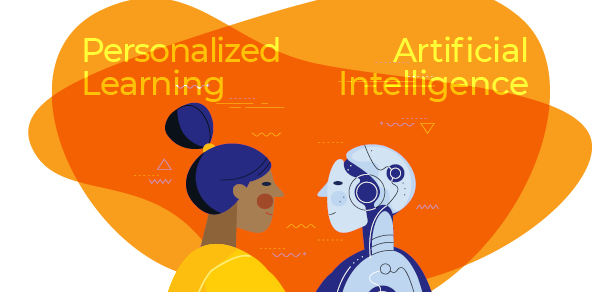
\includegraphics[width=\linewidth]{images/personalized_education.jpg}
    \caption{Ilustração de educação personalizada\cite{i33}}
    \vspace{4mm}
    \label{personalized_education}
\end{wrapfigure}
%
Nem todos os alunos assimilam o conhecimento da mesma forma. Alguns captam informação mais rapidamente, enquanto que outros precisam de mais tempo. O sistema de educação tradicional falha em oferecer uma abordagem personalizada, e de certa forma, equitativa. Cada aluno é singular. É neste caso que a \ac{ia} emerge na educação como solução
\par
A \ac{ia} no setor educacional assegura a personalização do software educativo para cada aluno. Adicionalmente, através de tecnologias complementares como machine learning na educação, o sistema é capaz de monitorizar como o aluno assimila diferentes lições e se ajusta a esse processo para mitigar qualquer dificuldade.

%%% Assistência 24/7 %%%
\subsubsection{Assistência constante}
Os chatbots\footnote{Software baseado numa inteligência artificial} representam um exemplo cada vez mais presente de como a \ac{ia} na educação utiliza dados para informar e oferecer assistência de maneira personalizada.
\par
Na esfera educacional, a \ac{ia} proporciona tutoria inteligente ao analisar de perto os padrões de consumo de conteúdo e ao se adaptar às necessidades individuais de cada aluno. Em um cenário global em que a aprendizagem remota e cursos de treinamento corporativo ganham destaque, possibilitando que as pessoas não interrompam as suas atividades quotidianas, os chatbots de \ac{ia} são destacados, por solucionarem duvidas sobre matrículas, oferecer respostas imediatas, fornecer acesso a materiais de estudo essenciais e prestar assistência 24 horas por dia, 7 dias por semana.

\subsection{Desvantagens}
\subsubsection{Ameaça ao estado laboral dos professores}
Apesar de ainda não se verificar, há a preocupação de que o avanço e a adoção da inteligência artificial possam influenciar a necessidade de certas funções no âmbito educacional. À medida que a \ac{ia} continua a automatizar mais facetas do processo educativo, é possível que haja uma redução na procura por educadores humanos, o que poderia resultar tanto numa melhoria da produtividade como em potenciais perdas de emprego.

\subsubsection{Dependência de tecnologia}
À medida que as escolas se tornam cada vez mais dependentes de soluções alimentadas por inteligência artificial, existe o risco de que professores e alunos possam depender demasiado da tecnologia. A longo prazo, essa dependência poderia resultar na negligência de métodos de ensino tradicionais importantes e no desenvolvimento de habilidades críticas de pensamento e resolução de problemas.


\subsection{Preocupações}
Apesar de tudo, a rápida evolução da tecnologia traz consigo vários riscos e desafios que, até ao momento, ultrapassaram as discussões e os enquadramentos regulatórios. A UNESCO está empenhada em auxiliar os Estados Membros na exploração do potencial das tecnologias de IA para alcançar os objetivos da \href{https://www.unesco.org/sdg4education2030/en}{Agenda 2030} para a Educação. Ao mesmo tempo, a UNESCO visa garantir que a integração da \ac{ia} em contextos educacionais seja orientada por princípios fundamentais de inclusão e equidade.\cite{ai_education}


%%%%% Serviços Empresariais %%%%%
\section{Serviços Empresariais}
É crucial que as empresas encarem a \ac{ia} não apenas como uma nova tecnologia, mas sim como uma ferramenta para fortalecer as capacidades empresariais. De forma geral, a \ac{ia} pode satisfazer algumas necessidades essenciais: automatizar processos, fornecer uma visão cognitiva e envolver clientes e colaboradores, etc.

% Tabela com o tabularrray (os docs eram bastantes simples de seguir, depois vê comigo isto, não sei se ha outra opção mais simples) https://ctan.org/pkg/tabularray?lang=en
\begin{table}[h]
  \centering
  \setlist{nosep, itemsep=1pt, leftmargin=*}
  \begin{tblr}{
      hlines, vlines,
      colspec = {X[0.5,l, m] X[1.5,l,m]},
      stretch = -1,
      row{1}  = {c, font=\bfseries},
      rowsep  = 5pt,
      measure = vbox,
  }
    Necessidades das Empresas & Tarefas e Aplicações            
    \\
    Visão cognitiva &
    \begin{itemize}
        \item Prever o que um determinado cliente é suscetível de comprar;
        \item Identificar a fraude de crédito em tempo real e detetar fraudes em reclamações de seguros;
        \item Automatizar a segmentação personalizada de anúncios digitais.
    \end{itemize}   
    \\
    Disponibilidade e suporte &
    \begin{itemize}
        \item Suporte instantâneo e personalizado;
        \item Resolução rápida de consultas frequentes, melhorando a experiência do cliente e reduzindo tempos de espera;
        \item Monitorização das redes sociais e outras plataformas para análise de sentimento.
    \end{itemize}   
    \\
    Automatização de processos &
    \begin{itemize}
        \item Correção de falhas na cobrança de serviços através de sistemas de faturação, ao extrair informação de múltiplas fontes;
        \item Leitura de documentos legais e contratuais para extrair provisões, utilizando processamento em linguagem natural.
    \end{itemize}   
    \\
    Velocidade &
    \begin{itemize}
        \item Processamento instantâneo de grandes volumes de dados para análise em tempo real;
        \item Atuação eficiente em cenários de rápida mudança, como no acompanhamento dinâmico de notícias.
    \end{itemize}
    \\
    Inovação &
    \begin{itemize}
        \item A capacidade de analisar rapidamente vastas quantidades de dados pode resultar em ofertas de produtos e serviços únicas e inovadoras que ultrapassam a concorrência.
    \end{itemize}
    \\
  \end{tblr}
  \caption{Tabela de Necessidades das Empresas e respetivas Tarefas/Aplicações.}
  \label{necessities_tabel}
\end{table}
%
%
%%%%%%%%%%%% Aspetos Éticos %%%%%%%%%%%%
%
\chapter{Aspetos Éticos}
\label{chap.aspetos_eticos}
%%%%% Na atualidade %%%%%
\section{Atualidade}
%
Na atualidade, testemunhamos o crescimento da \ac{ia}, uma revolução tecnológica que redefine os limites da inovação e da automação da vida humana. À medida que a \ac{ia} se torna uma peça central nos vários momentos do nosso dia a dia, desde assistentes virtuais até sistemas de tomada de decisões complexas, tornando-se assim inevitável questionar-nos a nós mesmo não apenas o seu potencial, mas também os dilemas éticos que a acompanham.
\par
Até que ponto a coleta e o uso de dados pela \ac{ia} respeitam a privacidade individual? Quem é responsável por ações tomadas por sistemas de \ac{ia} autónomos? Estas perguntas são exemplos de questões que surgem quanto a este assunto. Será mesmo seguro a utilização da \ac{ia}? 
\par
\par
\begin{figure}[ht]
    \centering
    \includegraphics[width=0.8\textwidth]{images/touchai.jpg}
    \caption{Ilustração da interação do homem com \ac{ia}\cite{i41}}
    \label{touchai}
\end{figure}

%%%PRIVACIDADE%%%
\section{Privacidade}
%%%
A \ac{ia} lida frequentemente com a análise e processamento de dados pessoais sensíveis. O uso indiscriminado ou inadequado desses dados pode comprometer a privacidade individual do utilizador, expondo assim informações pessoais em contextos inseguros ou a usos não autorizados. Combater essa privacidade torna-se uma das prioridades principais dos desenvolvedores enquanto ocorre o avanço da \ac{ia}. Para isso é crucial estabelecer protocolos robustos de colheita, armazenamento e compartilhamento de dados, garantindo que os usuários sejam plenamente informados sobre como as suas informações serão utilizadas, designado também por cookies\cite{privacidade}.
\par
\begin{figure}[ht]
    \centering
    
\includegraphics[width=1\textwidth]{images/privacidade.jpg}
    \caption{Ilustração da privacidade do utilizador.\cite{i42}}
    \label{privacidade}
\end{figure}
O consentimento informado deve ser obtido de maneira clara e transparente ao utilizador através de mensagens objetivas, permitindo que a pessoa que use tenha controle sobre o uso das suas informações pessoais. Além disso, a implementação de medidas de segurança rigorosas, como a anonimização de dados sempre que possível, é essencial para prevenir violações de privacidade dos seus utilizadores. O equilíbrio entre a necessidade de dados para o desenvolvimento da \ac{ia} e a proteção da privacidade individual é um desafio ético contínuo que requer atenção cuidadosa e regulamentação adequada dos seus desenvolvedores.  
%
\section{Responsabilidade}
A responsabilidade ética na \ac{ia} refere-se à obrigação moral e legal dos criadores, desenvolvedores e implementadores de sistemas de \ac{ia} em garantir que essas tecnologias sejam utilizadas de maneira ética e benéfica para o resto da nossa sociedade. 
\par
Alguns aspetos essenciais relacionados com a responsabilidade ética na \ac{ia} são \cite{responsabilidade}:
\begin{enumerate}
    \item \textbf{Tomada de decisões transparentes:} A responsabilidade começa com a transparência na tomada de decisões. Desenvolvedores de \ac{ia} devem assegurar que os processos que decidem os algoritmos sejam compreensíveis, permitindo que usuários e partes interessadas entendam como as decisões são alcançadas. 
    \item \textbf{Consciência do contexto social:} Desenvolvedores têm a responsabilidade de compreender o contexto social em que a \ac{ia} é aplicada. Isso inclui considerar os impactos sociais, culturais e económicos de suas tecnologias, bem como abordar questões éticas específicas a esses contextos. 
    \item \textbf{Ética na pesquisa e desenvolvimento: }A ética deve ser incorporada desde as fases iniciais da pesquisa e desenvolvimento. Isso inclui a escolha ética de conjuntos de dados, métodos de treinamento e a definição de objetivos para garantir que a \ac{ia} seja desenvolvida e aplicada de maneira ética desde o início até ao fim.
\end{enumerate}

%%%TRANSPARENCIA%%%
\section{Transparência}
%%%
A transparência e explicabilidade\footnote{Capacidade e qualidade de explicar um certo assunto de forma clara} na \ac{ia} referem-se à capacidade de compreender e explicar as decisões tomadas por algoritmos e devem ser o mais simples possível, garantindo que esses processos sejam claros e compreensíveis para os usuários e demais partes interessadas. Um exemplo dos pontos essenciais sobre esse aspeto crítico da ética em \ac{ia} é a explicação da resposta dada. Ou seja, a transparência começa com a capacidade de compreender como um sistema de \ac{ia} chega a suas decisões. Os usuários devem ter uma visão clara do processo decisório, desde a entrada de dados até a saída resultante. Como, por exemplo no auxílio na resolução de problemas, evitando assim que o output seja unicamente a resposta, mas sim a mesma e a explicação de como chegou á resposta correta.
\par
\begin{figure}
    \centering
    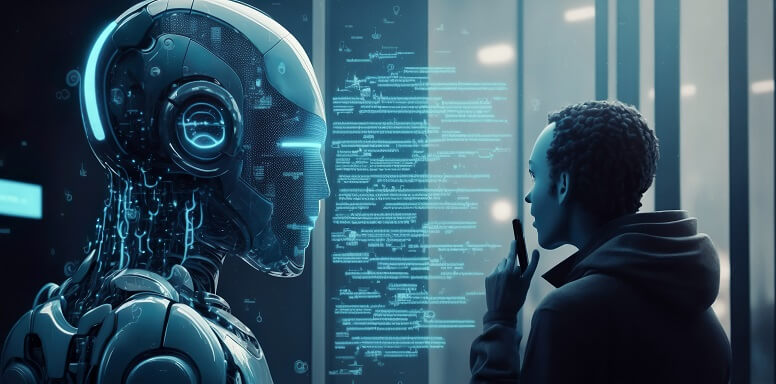
\includegraphics[scale=0.5]{images/ajuda_da_IA.jpg}
    \caption{Ilustração do auxílio da IA nas tarefas humanas\cite{i43}}
    \label{ajuda_da_IA}
\end{figure}

%%%USO MILITAR%%%
\section{Uso militar}
%%%
Devido ao aumento da utilização da \ac{ia} em várias setores, o contexto militar não foi exceção o que levanta diversas questões éticas nomeadamente à letalidade destas ferramentas. Alguns aspetos éticos são: 
\begin{enumerate}
    \item \textbf{Decisões autónomas:} A capacidade de sistemas de \ac{ia} tomar decisões autónomas no campo de batalha levanta preocupações sobre a responsabilidade e a falta de controle humano nas operações militares.
    \item \textbf{Ética na escolha de alvos:} A precisão na seleção de alvos é crucial. O uso de \ac{ia} em sistemas de armas deve garantir a conformidade com o direito internacional humanitário, evitando ataques indiscriminados e minimizando danos colaterais.
\end{enumerate}
\newpage
\par
A criação de novas armas que incorporem a \ac{ia} é um tópico que gera um debate ético onde existe pessoas que defendem essa ideia, porém existe também uma grande parte da nossa sociedade que abomina esse assunto. Estes são alguns exemplos de armas que possuem \ac{ia}:
\par
\begin{enumerate}
    \item \textbf{Drones:} Estes podem ser conduzidos a vários quilómetros de distância sendo os mesmos letais nos seus ataques.
    \begin{figure}[ht]
    \centering
    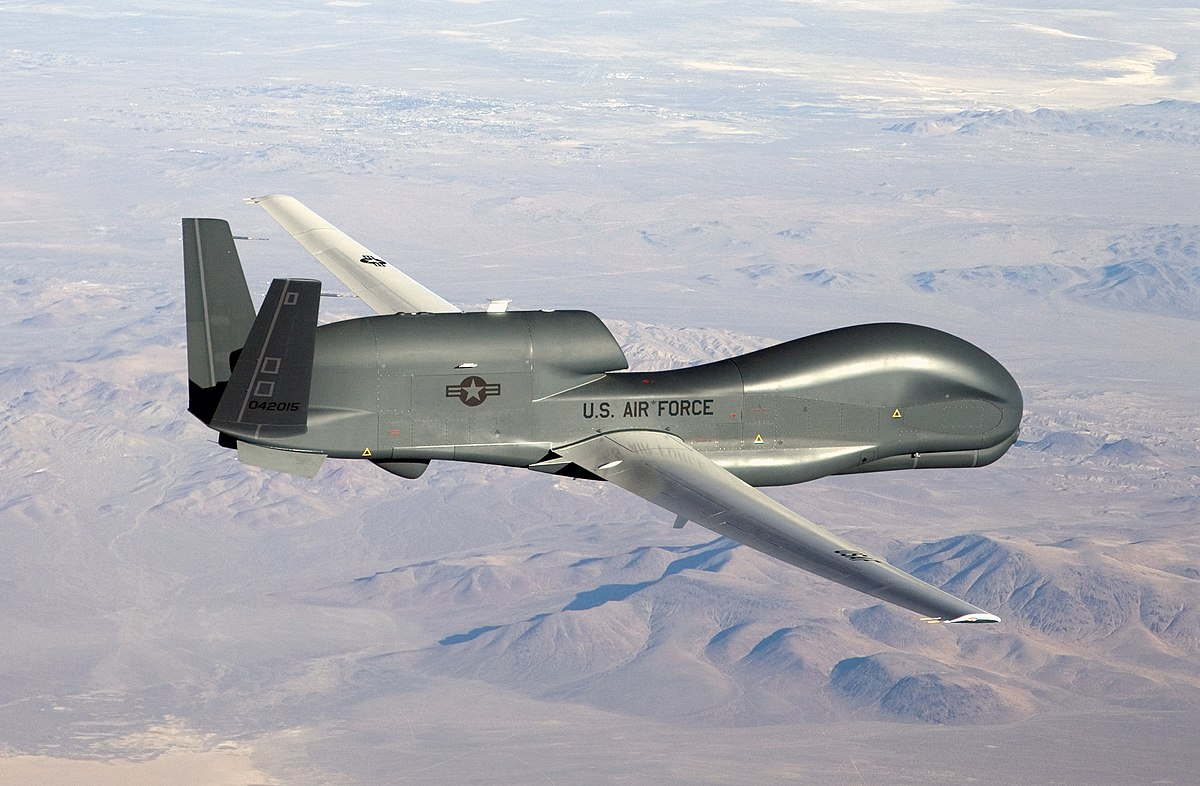
\includegraphics[width=0.75\textwidth]{images/RQ_04.jpg}
    \caption{Modelo RQ4 Global Hawk\cite{i44}}
    \label{RQ_04}
    \end{figure}
    \item \textbf{Sistemas de defesa área}: Cada vez mais usados pelos países para se defenderem dos ataques aéreos de outros países. Estas defesas são bastantes eficazes e capazes de defenderem o seu país de vários mísseis em simultâneo.
    \begin{figure}[ht]
    \centering
    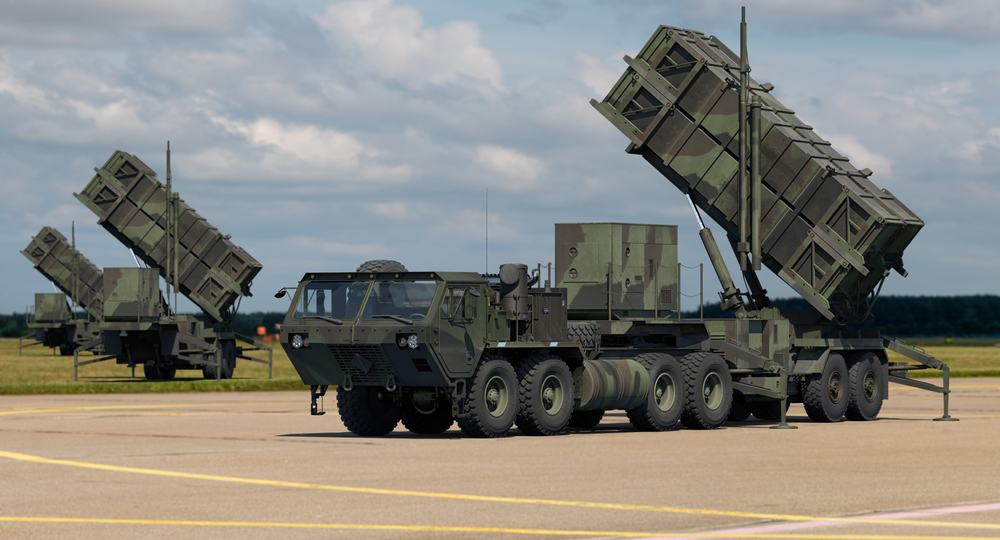
\includegraphics[width=0.75\textwidth]{images/sistema_patriot.jpg}
    \caption{Defesa antiaérea Patriot\cite{i45}}
    \label{sistema_patriot}
    \end{figure}
\end{enumerate}
%
%%SISTEMAS DE JUSTIÇA%%%
\section{Sistemas de justiça}
%%%
O uso da inteligência artificial está a aumentar nos sistemas de justiça, o que remete para um aumento na confiança do homem na mesma. Isaac Asimov criou 3 leis 
robóticas, afirmando que a utilização da \ac{ia} tinha de cumprir as mesmas. 
%
\begin{figure}[ht]
\centering
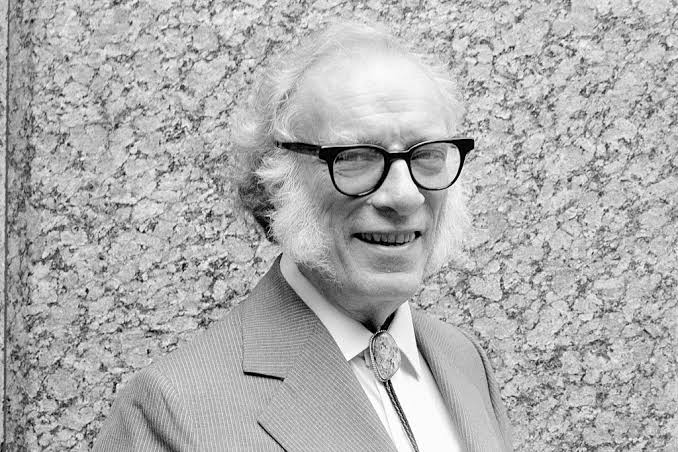
\includegraphics[width=0.75\textwidth]{images/images.jpeg}
\caption{Isaac Asimov\cite{i46}}
\label{Isaac Asimov}
\end{figure}
\par
\par
As três leis robóticas ditas por Isaac Asimov \cite{isaac} 
\begin{enumerate}
    \item \textbf{Não prejudica:} um robô não pode magoar um ser humano ou permitir que um ser humano sofra algum mal por inação. 
    \item \textbf{Obediência:} Um robô deve obedecer às ordens dos seres humanos, a menos que essas ordens entrem em conflito com a primeira lei.
    \item \textbf{Auto proteção:} um robô deve proteger a sua própria existência, desde que isso não entre em conflito com a primeira ou segunda regra.
\end{enumerate}
%


%
%%%%%%%%%%%
%
\chapter{Conclusão}
\label{chap.Conclusão}
O panorama futuro da inteligência artificial é bastante promissor. À medida que a \ac{ia} evolui, torna-se crucial para os profissionais estarem atualizados e cientes das tendências emergentes. A inteligência artificial (IA) emergiu como uma força transformadora na sociedade contemporânea, remodelando fundamentalmente a maneira como interagimos, trabalhamos e percebemos o mundo ao nosso redor. Este trabalho explorou as diversas facetas da IA, desde suas origens históricas até às suas aplicações práticas e implicações éticas. Ao analisar a evolução da IA, torna-se evidente que estamos a testemunhar uma revolução tecnológica que rivaliza com as grandes transformações da história humana.
\par
A capacidade da \ac{ia} de aprender, adaptar-se e tomar decisões autónomas introduz novas dimensões na solução de problemas complexos. No entanto, à medida que confiamos cada vez mais nas capacidades desta tecnologia, surgem questões éticas cruciais. A transparência, a responsabilidade e a equidade tornam-se imperativos incontestáveis.
\par
Além disso, a interação harmoniosa entre humanos e sistemas de IA é essencial para maximizar os benefícios potenciais dessa tecnologia. A relação simbiótica, onde a inteligência artificial complementa as habilidades humanas, surge como um modelo promissor para o futuro. A capacidade de fusão entre intelectos humanos e algoritmos avançados pode resultar em inovações extraordinárias em campos como medicina, computação quântica, finanças, e educação.
\par
Em resumo, a inteligência artificial é uma ferramenta poderosa que está a moldar o curso da civilização moderna. Neste cenário em constante evolução, é essencial cultivar uma abordagem responsável, ética e colaborativa para garantir que a \ac{ia} contribui para o bem-estar global e a progressão sustentável da sociedade. A jornada da inteligência artificial é intrinsecamente vinculada à nossa capacidade de moldar o seu desenvolvimento e aplicação para alinhar-se aos valores humanos fundamentais.


\chapter*{Contribuições dos autores}
Cada autor contribuiu igualmente para o produto final do trabalho, sendo justamente atribuído a nota de 50\% a cada um. \\
O autor \ac{tm} realizou metade do capítulo de Percurso da Inteligência Artificial, o capítulo de Impacto nos Setores, Conclusão e Introdução. \\
O autor \ac{pl} realizou metade do capítulo de Percurso da Inteligência Artificial, e o capítulo de Aspetos Éticos.

\vspace{10pt}
\textbf{Percentagem de contribuição de cada autor.}\\

\ac{tm}, \ac{pl} : 50\%, 50\%\\

%%%%%%%%%%%%%%%%%%%%%%%%%%%%%%%%%
\chapter*{Acrónimos}
%
\begin{acronym}
\acro{ua}[UA]{Universidade de Aveiro}
\acro{leci}[LECI]{Licenciatura em Engenharia de Computadores e Informática}
\acro{tm}[TM]{Tiago Mendes}
\acro{pl}[PL]{Paulo Lacerda}
\acro{glisc}[GLISC]{Grey Literature International Steering Committee}
\acro{ia}[IA]{Inteligência Artificial}
\acro{gpt2}[GPT-2]{Generative Pre-trained Transformer 2}
\acro{gpt3}[GPT-3]{Generative Pre-trained Transformer 3}
\acro{xai}[XAI]{Explainable Artificial Intelligence}
\acro{qml}[QML]{Quantum Machine Learning}
\end{acronym}


%%%%%%%%%%%%%%%%%%%%%%%%%%%%%%%%%
\printbibliography
\end{document}